\entry{2026-10-09}{Wider bank (C1, complete): memory wall gone, accuracy gain not yet}

Lane \texttt{2026-10-08-jcp-wide-bank} (last commit \texttt{2c3c397e0}, mirror \texttt{dbb3da96f}). Jobs 5012313, 5012763 (A100); 5012847, 5022387 (H200); 5020724, 5020855, 5021867, 5022113 (H100). Every step was Codex-gated, and the final report audit says REPORT-OK. Report: \path{worktrees/2026-10-08-jcp-wide-bank/experiments/jcp-wide-bank/report.md}. \textbf{Provisional:} first-order references, and the 3D selections are post hoc (A7). The J4 solver uses 6 adaptive steps (A8), so J4 is not comparable with earlier 3D runs.

\subsection*{Findings}
\begin{itemize}
\item \textbf{2D dial stops at $R'=384$.} Against the space-only reference, the worst error falls 3.45 $\to$ 1.49 $\to$ 1.05\,\% for $R'=128 \to 256 \to 384$, but $R'=512$ is worse on 28 of 38 cases at 3.4$\times$ the cost. Against the space+time reference the median is flat at 0.91\,\%, consistent with time-step error dominating (a hypothesis).
\item \textbf{Test-count trim does not work.} The registered mechanism is contradicted in 2D and 3D; only one 2D trim gives a 25\,\% saving for a negligible ST change.
\item \textbf{Wider 3D bank ($R=1024$) trained.} Its worst projection floor falls 3.23 $\to$ 1.93 $\to$ 1.29\,\% for $R'=512 \to 768 \to 1024$.
\item \textbf{But the 3D ROM barely follows.} From $R'=512$ to 1024 every case improves slightly, yet the median stays near 1.1\,\% and the worst error is non-monotone (about 3.4--4.4\,\%). The registered verdict is \emph{unavailable}, because a quadrature-convergence gate fails at $R' \ge 768$.
\item \textbf{The memory wall is gone.} At $R'=1024$ the off-mesh rule needs 1.61\,GB, against 34.37\,GB for the tensor.
\end{itemize}
\begin{center}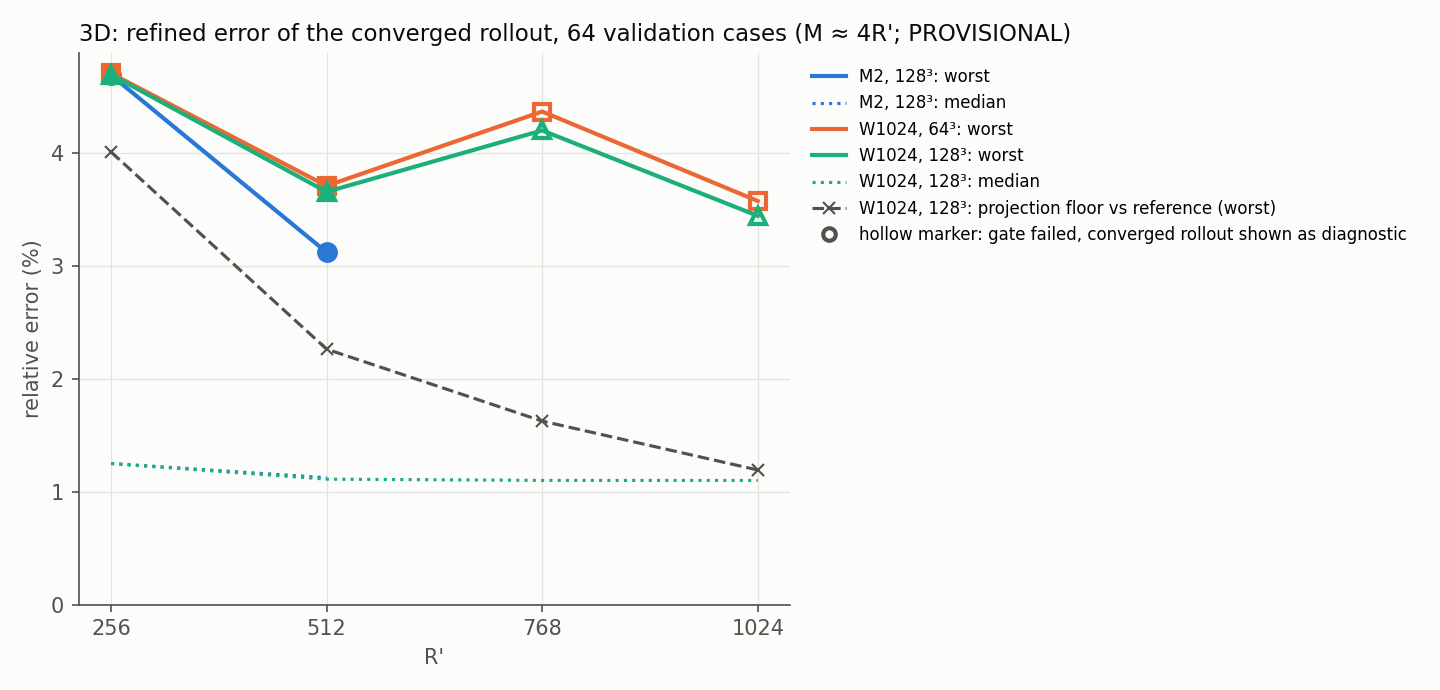
\includegraphics[width=0.75\linewidth]{figs/c1_3d_j4_error_vs_Rp.png}\end{center}
\begin{center}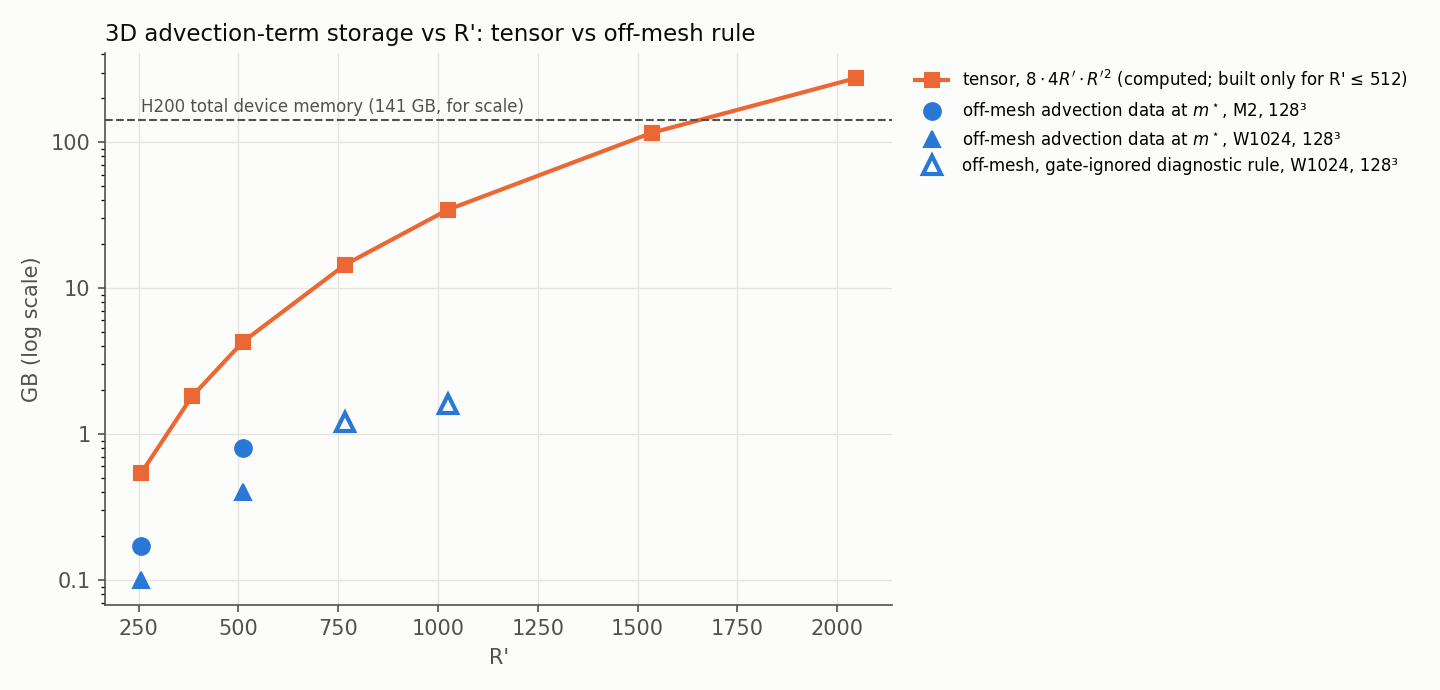
\includegraphics[width=0.75\linewidth]{figs/c1_3d_j4_memory_vs_Rp.png}\end{center}

\subsection*{Retracted}
\retracted{the 4-case preview of 1.43\,\% worst error at $R'=1024$, $128^3$ (relayed on 2026-10-08) did not hold on all 64 cases: the full-cohort worst is about 3.4\,\%. ``The 2D dial extends to 512'' and the registered test-count-trim mechanism are both retracted.}

\subsection*{What it means}
The bank is no longer the bottleneck: the reduced model sits well above the bank's projection floor. With C2 (time error dominates) and C3 (smoother or Sobolev banks do not help the ROM), the evidence points to time discretisation and the first-order reference as the next limits. The obvious next experiment is second-order stepping with the wide bank, against second-order references.
